\documentclass{article}

\author{Tran Van Tan Khoi}

\date{May 14, 2025}

\title{Weekly Homework Report \#6}

\usepackage[utf8]{inputenc}
\usepackage[a4paper,top=2cm,bottom=2cm,left=3cm,right=3cm,marginparwidth=1.75cm]{geometry}
\usepackage[colorlinks=true, allcolors=blue]{hyperref}
\usepackage{graphicx}

\begin{document}

\maketitle

\section{Introduction}
\label{introduction}

It is typical for people wanting to ask questions (or in more technical terms, `make queries') about whether an object or item exists in a set or a container. For basic use case, arrays and linked lists are perfectly capable of answering such requests in $O(n)$ (or $O(\log n)$ if the array is sorted). But if the objects aren't necessarily comparable (i.e. no ordering properties) then there is a better solution: hash map (or hash table) - converting huge amount of data into a short identifying string of characters and digits. Not only this is still used in modern architecture, there is an entire field dedicated to this philosophy: \emph{Cryptography}.

In this homework, we will apply the hash map data structure to a given problem and analyze why it is useful in many situations. The source code and this report can be found on \href{https://github.com/xtrkoi/throwaway-rep}{Github}.

\begin{figure*}[h]
    \centering
    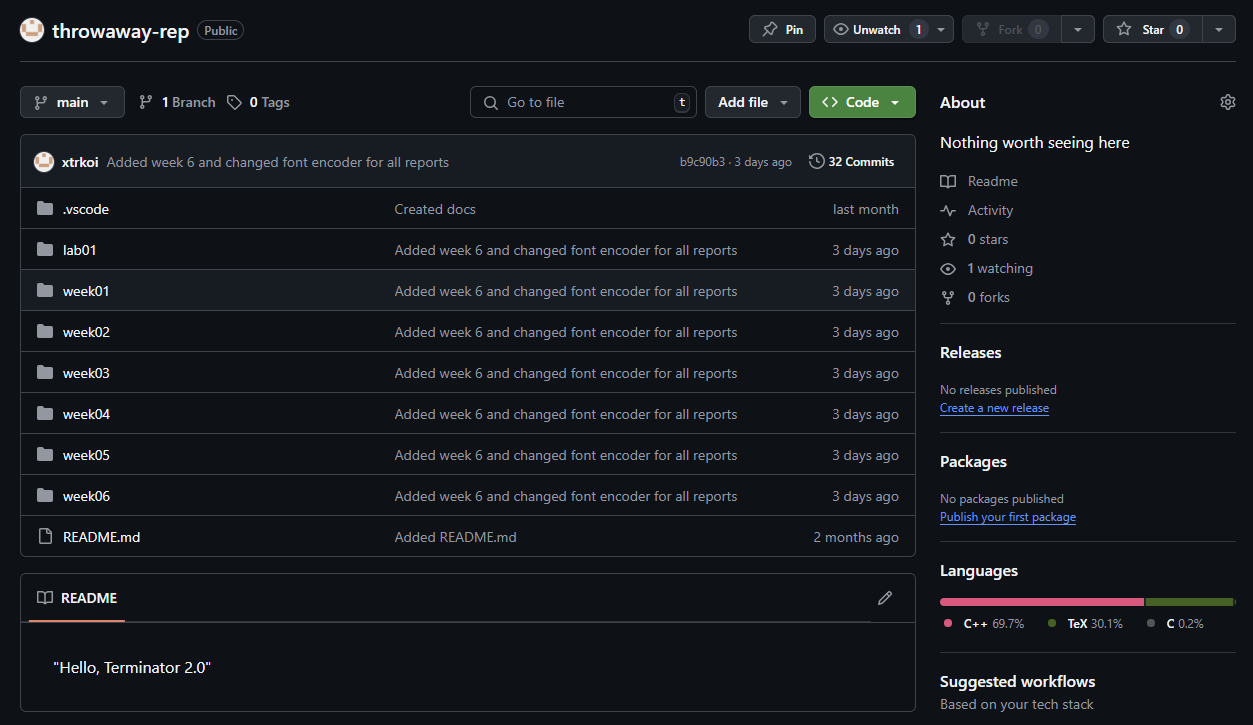
\includegraphics[width=12cm]{images/github_page.png}
\end{figure*}

\section{Problem}
\label{problem}

We are given a list of companies with their profit tax codes and addresses on multiple lines. We will store all the companies' information and get the full information of a company using just their name. The time complexity for both operation (inserting and querying a single company) will be constant time $O(1)$, assuming the time to process a company's information is insignificant, and with some caveats.

\section{Solution}
\label{solution}

We will use an array to store the information, but instead of in increasing order of indices ($i=0, 1, 2, 3, ...$), we will find the index where each item will go using a specific hashing function.

Assuming each company's name is distinct, we can encode the name into a hash integer ($< 2000$) with high probability of being unique from other created hashes. To do this, we employ \emph{polynomial rolling hash function}, a hashing algorithm that creates hashes based on the specific character at a position.

However, any hash function has a flaw: it can create same hash for different items. This is called a \emph{collision} and there are methods of resolving these. Here we will use the simplest and understandably the worst: \emph{Linear Probing}. If we created a hash that is already existed, we will traverse the entire map in each step to find the next empty slot.

\section{Analysis}
\label{analysis}

The greatest advantage of hashing over elementary data structures is speed. With a well-designed hash function and a good collision resolution strategy, both insertion and lookup operations can be performed in constant average time, $O(1)$. This is a significant improvement over linear data structures like arrays or linked lists, where such operations may require $O(n)$ time.

However, the efficiency of a hash map depends on several factors:
\begin{itemize}
    \item \emph{Hash Function Quality:} A poor hash function can lead to many collisions, degrading performance to $O(n)$ in the worst case.
    \item \emph{Load Factor:} As the number of stored items approaches the size of the hash table, the probability of collisions increases, which can also reduce performance.
    \item \emph{Collision Resolution:} The chosen method (e.g., linear probing, chaining) affects both speed and memory usage.
\end{itemize}

Here, we used a polynomial rolling hash function, which distributes company names uniformly across the table with high probability. Linear probing is used for collision resolution, which is simple but can suffer from clustering if the table becomes too full.

\section{Conclusion}
\label{conclusion}

We explored the use of hash maps for efficiently storing and retrieving company information by name, achieving constant average time complexity for both insertion and lookup operations. This demonstrates the practical advantages of hash maps over simpler data structures, especially when fast access is required. However, careful consideration must be given to the choice of hash function, collision resolution strategy, and table size to maintain optimal performance. Overall, hash maps are a powerful tool for managing large datasets where quick access is essential.

\end{document}